%%Énoncé
\begin{itemize}
\item Quels sont les avantages et inconvénients éventuels d’implémenter une file de priorité par un tas plutôt que par une liste ? (Mathieu)\newline

L'avantage principal de l'utilisation d'un tas pour implémenter une file de priorité plutôt qu'une liste est que les opérations d'insertion et de retrait d'entrées s'effectuent en $O(log(n))$. Les listes triées (resp. non triées) quant à elles effectuent les opérations d'insertions en $O(1)$ (resp. $O(n)$) et de retraits en $O(n)$ (resp. $O(1)$).\newline

De plus, l'opération de triage d'une file de priorité implémentée par un tas contenant une séquence de n éléments s'effectue en temps $O(n*log(n))$, là où une file de priorité implémentée par une liste contenant les mêmes éléments s'effectue en temps $O(n^2)$.\newline

\item Existe-t-il un tas T mémorisant 7 éléments distincts tel qu’un parcours infixe du tas renvoie les éléments de T en ordre décroissant ?\newline

Non, ce n'est pas possible étant donné que, selon la comparaison utilisée (directe ou inverse), l'entrée possédant la plus grande/la plus petite priorité est située à la racine de l'arbre représentant le tas. Etant donné qu'un parcours infixe commence par le noeud le plus à gauche de l'arbre et se termine par celui le plus à droite de l'arbre, les priorités des entrées ne peuvent être parcourues en ordre décroissant.\newline

\item Qu’en est-il avec un parcours préfixe ou post-fixe ?\newline

\begin{figure} [h]
	\centering
	\hspace{-6cm}
	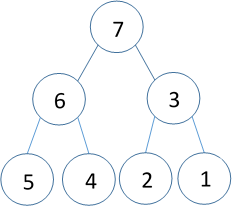
\includegraphics[scale=0.5]{ArbrePrefixe.png}
\end{figure}

\begin{figure} [h]
	\centering
	\vspace{-3.7cm}
	\hspace{6cm}
	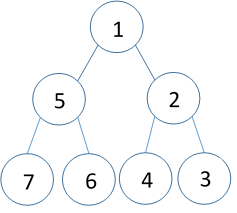
\includegraphics[scale=0.5]{ArbrePostfixe.png}
\end{figure}

L'arbre de gauche convient dans le cas d'un parcours préfixe, tandis que l'arbre de droite convient pour un parcours postfixe. Ici, les valeurs correspondantes aux clés de priorité sont ommises pour plus de clarté.\newline

Dans le premier cas d'un parcours préfixe (arbre de gauche), on parcours le noeud courant, puis son fils gauche et ensuite son fils droit. Dans le second cas du parcours postfixe, on parcours le fils gauche, le fils droit et ensuite on parcours le noeud courant. Dans les deux cas, on obtient bien la séquence 7-6-5-4-3-2-1.

\end{itemize}
%%Réponse
